\section{Room Driver}\label{sec:room-driver}
Room Driver zajišťuje komunikaci mezi službou Room Assistant a řídící jednotkou v kurníku.
Tato jednotka se stará o ovládání dveří, světla a poskytování dat o aktuální teplotě a vlhkosti.
Ovládání nízkoúrovňových komponent a komunikaci s připojeným počítačem zajišťuje Arduino Nano.
Arduino je připojeno pomocí USB sběrnice k počítači, který na základě domluvených pravidel jednoduchého komunikačního protokolu posílá znaky, na které Arduino příslušně reaguje dle programu.
Tato služba má tedy za úkol přes sériové rozhraní posílat příkazy a načítat stavy řídící jednotky na základě requestů přijmutých na REST API.

\subsection*{Popis algoritmu}
Po startu služby se nejdříve vytvoří instance třídy ArduinoReader.
Jedná se o vlastní třídu, při inicializaci vytvoří instanci sériového spojení k Arduinu.
Je zde implementován connection pool, který se stará o zdraví spojení po celou dobu běhu aplikace.
Třída má jedinou metodu, a tou je run\_command.
Tato metoda přijímá jako parametr jeden znak, který při provolání metody pošle zkrze sériové připojení do Arduina a vrátí data typu String, kterými odpoví Arduino zpět.
Jakmile se povede provést inicializaci sériového spojení je spuštěno REST API.
Toto API poskytuje endpointy pro vyslání příkazů k zavření a otevření dvířek, zhasnutí a rozsvícení světla, informací o aktuálních stavech jednotky a informací o teplotě a vlhkosti v kurníku.
Informace o aktuálním stavu jsou dobré pro případ, kdy se budou muset služby restartovat a bude třeba načíst reálný aktuální stav.
V případě, kdy přijde požadavek na konkrétní endpoint, jako první věc se provede odeslání příslušného znaku jako příkaz Arduinu.
Následně se počká na jeho odpověď, pokud je požadavek typu POST.
Odpověď je následně převedena do JSON objektů a vrácena v HTTP odpovědi s typem těla odpovědi JSON.

\subsection*{Příkazy ovládacího protokolu}
\begin{itemize}
    \item o = otevřít dvířka
    \item c = zavřít dvířka
    \item l = rozsvítit světlo
    \item d = zhasnout světlo
    \item j = vrátí zprávu ve formátu JSON s daty o teplotě a vlhkosti
    \item s = vrátí zprávu ve formátu SJON s daty o stavech jednotlivých ovládaných prvků (dveře, světlo)
\end{itemize}


(obrázek \ref{fig:homeasistant_temperature}).

\begin{figure}[H]
    \centering
    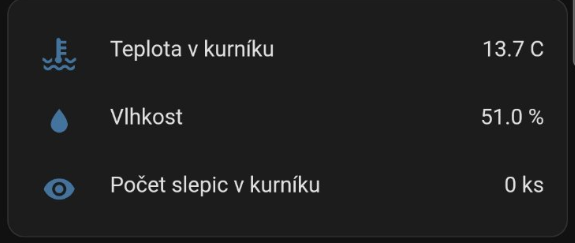
\includegraphics[width=0.8\textwidth]{img/homeasistant_temperature.png}
    \caption{Vizualizace dat ze senzoru v systému Home Assistant}
    \label{fig:homeasistant_temperature}
\end{figure}


%# coopmaster-room-driver
%
%Aplikace provazuje core aplikace(konkrétně službu room assistant) s arduinem ovladajicim svetla, dvere a poskytujici informaci o teplote a vzdusne vlhkosti.
%Součástí projektu je i firmware arduina.

%## funkcionalita
%- umoznuje ovladat osvetleni kurniku
%- resi otevírání a zavírání dvířek v kurníku
%- ziskava informace ze senzoru o teplote a vlhkosti v kurniku
%- komunikuje se zbytkem systému pomocí rest api
%- s arduinem komunikuje pomocí serialového portu a pomocí zasílání příkazů v podobě jednoho písmene
%- příkazy: o = otevřít dvířka, c = zavřít dvířka, l = rozsvítit světlo, d = zhasnout světlo, j = vrátí json s daty o teplotě a vlhkosti, s = vrátí json s daty o stavech jednotlivých ovládaných prvku (dvěře, světlo)
%
%## technologie
%- python
%- knihovny pro python
%- **Flask**: Lehký webový framework, flexibilní a rychlý vývoj webových aplikací.
%- **colorama**: Manipulace s barvami v textovém výstupu na terminálu.
%- **waitress**: Rychlý WSGI server pro produkční nasazení webových aplikací.
%- **requests**: Jednoduché HTTP požadavky (GET, POST, atd.).
%- **Werkzeug**: WSGI nástroje pro webové aplikace (routování, správa relací).
%- **python-dotenv**: Načítání konfigurace z `.env` souborů.
%- **pyserial**: Komunikace se sériovými zařízeními přes sériové porty.
